% Created 2023-09-18 Mon 10:36
% Intended LaTeX compiler: pdflatex
\documentclass[11pt]{article}
\usepackage[utf8]{inputenc}
\usepackage[T1]{fontenc}
\usepackage{graphicx}
\usepackage{longtable}
\usepackage{wrapfig}
\usepackage{rotating}
\usepackage[normalem]{ulem}
\usepackage{amsmath}
\usepackage{amssymb}
\usepackage{capt-of}
\usepackage{hyperref}
\usepackage{pgfplots}
\pgfplotsset{compat=1.18}
\author{Hankertrix}
\date{\today}
\title{Math Module 3A Cheat Sheet}
\hypersetup{
 pdfauthor={Hankertrix},
 pdftitle={Math Module 3A Cheat Sheet},
 pdfkeywords={},
 pdfsubject={},
 pdfcreator={Emacs 29.1 (Org mode 9.6.6)}, 
 pdflang={English}}
\begin{document}

\maketitle
\setcounter{tocdepth}{2}
\tableofcontents

\newpage

\section{Definitions}
\label{sec:org0ee7176}

\subsection{Corollary}
\label{sec:org3fdd1f9}
A corollary is a proposition that is inferred immediately from a proved proposition with little or no additional proof.

\subsection{Lagrange's mean value theorem (MVT)}
\label{sec:org9039de0}
Suppose that:
\begin{enumerate}
\item \(f\) is continuous on a closed interval \([a, b]\)
\item \(f\) is differentiable on the open interval \((a, b)\)
\end{enumerate}

Then there is a point \(c \in (a, b)\) such that:
\[f'(c) = \frac{f(b) - f(a)}{b - a}\]

For an illustration of this theorem, go to \href{https://www.desmos.com/calculator/humyjrcbm4}{this link.}

\subsubsection{Corollaries}
\label{sec:orged0e5f8}
\begin{itemize}
\item If \(f'(x) = 0\) on an interval, then \(f\) is constant on the interval.
\item If \(f' = g'\) on an interval, then \(f = g + C\), where \(C\) is some constant.
\end{itemize}

\subsection{Rolle's theorem}
\label{sec:orgef10361}
Suppose that:
\begin{enumerate}
\item \(f\) is continuous on a closed interval \([a, b]\)
\item \(f\) is differentiable on the open interval \((a, b)\)
\item \(f(a) = f(b)\)
\end{enumerate}

Then there exists a point \(c \in (a, b)\) such that \(f'(c) = 0\).

\newpage

\subsection{Cauchy's mean value theorem}
\label{sec:orgb1cb532}
\begin{enumerate}
\item \(f\) and \(g\) are continuous on a closed interval \([a, b]\).
\item \(f\) and \(g\) are differentiable on the open interval \((a, b)\).
\end{enumerate}

Then there exists \(c \in (a, b)\) such that:
\[g'(c)[f(b) - f(a)] = f'(c)[g(b) - g(a)]\]

With \(g'(c) \neq 0\), \(g(b) - g(a) \neq 0\), we get:
\[\frac{f(b) - f(a)}{g(b) - g(a)} = \frac{f'(c)}{g'(c)}\]

With \(g(x) = x\), we get Lagrange's mean value theorem.

\subsection{Indeterminate forms}
\label{sec:orgab9818f}
If \(\lim_{x \rightarrow a} f(x) = \lim_{x \rightarrow a}g(x) = 0\), the limit \(\lim_{x \rightarrow a} \frac{f(x)}{g(x)}\) is called an \textbf{indeterminate form of type} \(\left[\frac{0}{0} \right]\).
\\[0pt]

Likewise, if \(\lim_{x \rightarrow a \pm} f(x) = \pm \infty, \ \lim_{x \rightarrow a \pm} g(x) = \pm \infty\), the limit \(\lim_{x \rightarrow a} \frac{f(x)}{g(x)}\) is called an \textbf{indeterminate form of type} \(\left[ \frac{\infty}{\infty} \right]\).

\subsubsection{More examples}
\label{sec:org12f547b}
\begin{enumerate}
\item \(\lim_{x \rightarrow 0} x \cdot \ln x\) produces the indeterminate form \([\infty \cdot 0]\).
\item \(\lim_{x \rightarrow \infty} (\sqrt{n^2 + 2n} - n)\) produces the indeterminate form \([\infty - \infty]\).
\item \(\lim_{x \rightarrow +\infty} \left(1 + \frac{1}{x} \right)^x\) produces the indeterminate form \([1^{\infty}]\).
\end{enumerate}

\newpage

\subsection{L'H\(\text{\^o}\)pital's Rule}
\label{sec:orgb2bec24}
If there exists \(\delta > 0\) such that:
\begin{enumerate}
\item \(f(x)\) and \(g(x)\) are differentiable on \((a - \delta, a) \cup (a, a + \delta)\)
\item \(g'(x) \neq 0\) on \((a - \delta, a) \cup (a, a + \delta)\)
\end{enumerate}

And also if:
\[\lim_{x \rightarrow a} f(x) = \lim_{x \rightarrow a} g(x) = 0\]

Then:
\[\lim_{x \rightarrow a} \frac{f(x)}{g(x)} = \lim_{x \rightarrow a} \frac{f'(x)}{g'(x)}\]

This only applies if the right-hand limit exists.

\subsubsection{The conditions, simplified}
\label{sec:orgc1e1de4}
\begin{enumerate}
\item \(\lim_{x \rightarrow a} \frac{f(x)}{g(x)}\) is of type \(\left[ \frac{0}{0}\right]\)
\item \(\frac{f'(x)}{g'(x)}\) makes sense for \(x\) close to \(a\), and has a limit as \(x \rightarrow a\).
\end{enumerate}

\subsubsection{Variations}
\label{sec:orgd7efa9d}
\[\text{1. } \lim_{x \rightarrow a+} \frac{f(x)}{g(x)} = \lim_{x \rightarrow a+} \frac{f'(x)}{g'(x)} \text{ if the right-hand side makes sense}\]
\[\text{2. } \lim_{x \rightarrow a-} \frac{f(x)}{g(x)} = \lim_{x \rightarrow a-} \frac{f'(x)}{g'(x)} \text{ if the right-hand side makes sense}\]
\[\text{3. } \lim_{x \rightarrow \pm \infty} \frac{f(x)}{g(x)} = \lim_{x \rightarrow \pm \infty} \frac{f'(x)}{g'(x)} \text{ if the right-hand side makes sense}\]

These rules \textbf{only apply} if the left-hand limit is an indeterminate form of the type \(\left[\frac{0}{0} \right]\) or \(\left[ \frac{\infty}{\infty} \right]\)

\subsubsection{Example 1}
\label{sec:org33bbc9f}
\begin{align*}
\lim_{x \rightarrow 0} \frac{e^x = 1}{\sin x} &= \lim_{x \rightarrow 0} \frac{e^x}{\cos x} \\
&= \frac{1}{1} \\
&= 1
\end{align*}

\subsubsection{Example 2}
\label{sec:org2e83b35}
\begin{align*}
\lim_{x \rightarrow +\infty} x^2 e^{-3x} &= \lim_{x \rightarrow +\infty} \frac{x^2}{e^{3x}} \\
&= \lim_{x \rightarrow +\infty} \frac{2x}{3e^{3x}} \\
&= \lim_{x \rightarrow +\infty} \frac{2}{9e^{3x}} \\
&= 0
\end{align*}

\subsubsection{Example 3}
\label{sec:org63a37bb}
\begin{align*}
\lim_{x \rightarrow +\infty} \left(1 + \frac{1}{x} \right)^{x} &= \lim_{x \rightarrow +\infty} e^{x \cdot \ln \left( 1 + \frac{1}{x} \right)} \\
&= e^{\lim_{x \rightarrow +\infty} x \cdot \ln \left(1 + \frac{1}{x} \right)}
\end{align*}

Finding the limit \(\lim_{x \rightarrow +\infty} x \cdot \ln \left(1 + \frac{1}{x} \right)\):
\begin{align*}
\lim_{x \rightarrow +\infty} x \cdot \ln \left(1 + \frac{1}{x} \right) &= \lim_{x \rightarrow +\infty} \frac{\ln \left(1 + \frac{1}{x} \right)}{\frac{1}{x}} \\
&= \lim_{x \rightarrow +\infty} \frac{\frac{1}{1 + \frac{1}{x}} \cdot \left( \frac{-1}{x^2} \right)}{\frac{-1}{x^2}} \\
&= \lim_{x \rightarrow +\infty} \frac{1}{1 + \frac{1}{x}} \\
&= \frac{1}{1 + 0} \\
&= 1
\end{align*}

Hence:
\begin{align*}
\lim_{x \rightarrow +\infty} \left(1 + \frac{1}{x} \right)^{x} &= e^{1} \\
&= e
\end{align*}

\newpage

\subsection{Convexity}
\label{sec:org7cf7896}
A function \(f(x)\) is called \textbf{convex} (or it is said to \textbf{concave upward}) on an interval \(I\) if for all \(a, b \in I\), the line segment joining the points \((a, f(a)), (b, f(b))\) lies above the graph of \(f(x)\).
\\[0pt]

\begin{center}
\begin{tikzpicture}
\begin{axis}
\addplot[color = blue]{- (x + 3) * (x - 3)};
\addplot[color = green]{-x};
\end{axis}
\end{tikzpicture}
\end{center}

A function \(f(x)\) is \textbf{convex} (or it is said to \textbf{concave upward}) on the interval \(I\) if and only if for any \(a < x < b\) in \(I\) we have:
\[\frac{f(x) - f(a)}{x - a} < \frac{f(b) - f(a)}{b - a}\]

\newpage

\subsection{Concavity}
\label{sec:org0f122a7}
A function \(f(x)\) is called \textbf{concave} (or it is said to \textbf{concave downward}) on an interval \(I\) if for all \(a, b \in I\), the line segment joining the points \((a, f(a)), (b, f(b))\) lies above the graph of \(f(x)\).
\\[0pt]

\begin{center}
\begin{tikzpicture}
\begin{axis}
\addplot[color = blue]{(x + 3) * (x - 3)};
\addplot[color = green]{x};
\end{axis}
\end{tikzpicture}
\end{center}

A function \(f(x)\) is \textbf{concave} (or it is said to \textbf{concave downward}) on the interval \(I\) if and only if for any \(a < x < b\) in \(I\) we have:
\[\frac{f(x) - f(a)}{x - a} > \frac{f(b) - f(a)}{b - a}\]

\newpage

\subsection{Inflection point}
\label{sec:orga30c384}
A point where the graph of a function has a tangent line and where the concavity changes, is called a \textbf{point of inflection} or an \textbf{inflection point}.

\subsubsection{Example}
\label{sec:orga3d4f34}
Both \(f(x) = x^3\) and \(f(x) =\sqrt[3]{x}\) have a point of inflection at \(x = 0\).
\\[0pt]

\begin{center}
\begin{tikzpicture}
\begin{axis}[axis lines = center, samples = 100, legend pos = north west]
\addplot[color = blue]{x^3};
\addlegendentry{$y = x^3$};
\addplot[color = red]{0};
\end{axis}
\end{tikzpicture}
\end{center}

\begin{center}
\begin{tikzpicture}
\begin{axis}[axis lines = center, samples = 100, legend pos = north west]
\addplot[color = blue]{x/abs(x) * abs(x)^(1/3)};
\addlegendentry{$y = \sqrt[3]{x}$};
\addplot[color = red]{0};
\end{axis}
\end{tikzpicture}
\end{center}

\newpage

\subsection{Second derivative}
\label{sec:orgd064f65}
Given a function \(f(x)\), its \textbf{second derivative} is the derivative of \(f'(x)\).

\subsection{Higher order derivatives}
\label{sec:org2ee7e95}
Given a function \(f(x)\), its \(n\)-th derivative is:
\[\underbrace{((f')' \cdots )'}_{n \text{ differentiations}}\]

\subsubsection{Standard notation}
\label{sec:orgaa3d224}
\begin{itemize}
\item \(f''\) for the second derivative
\item \(f'''\) for the third derivative
\item \(f^{iv}\) for the fourth derivative
\item \(f^{(n)}\) for the \(n\)-th derivative
\item \(C^n (A) = \{f: f^{(n)} \text{ exists and is continuous on } A\}\)
\end{itemize}

Note that:
\[C(A) \subset C'(A) \subset C''(a) \subset \ldots \subset C^{\infty} A\]

\newpage

\subsection{Vertical asymptote}
\label{sec:orgf988770}
The graph of \(y = f(x)\) has a \textbf{vertical asymptote} at \(x = a\) if:
\[\lim_{x \rightarrow a-} f(x) = \pm \infty \quad \text{or} \quad \lim_{x \rightarrow a+} f(x) = \pm \infty\]

\subsubsection{Example}
\label{sec:org55271b1}
\[f(x) = \frac{1}{x^2 - x}\]

The graph of \(f(x)\) has vertical asymptotes at \(x = 0\) and \(x = 1\).

\begin{center}
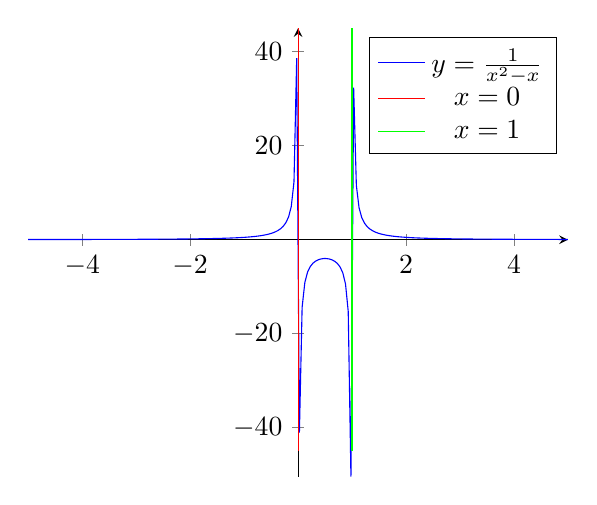
\begin{tikzpicture}
\begin{axis}[axis lines = center, samples = 200]
\addplot[color = blue]{1/(x^2 - x)};
\addlegendentry{$y = \frac{1}{x^2 - x}$};
\addplot[color = red] coordinates {(0, 45) (0, -45)};
\addlegendentry{$x = 0$};
\addplot[color = green] coordinates {(1, 45) (1, -45)};
\addlegendentry{$x = 1$};
\end{axis}
\end{tikzpicture}
\end{center}

\newpage

\subsection{Horizontal asymptote}
\label{sec:org36b1f44}
The graph of \(y = f(x)\) has a \textbf{horizontal asymptote} \(y = L\) if:
\[\lim_{x \rightarrow -\infty} f(x) = L \quad \text{or} \quad \lim_{x \rightarrow +\infty} f(x) = L\]

\subsubsection{Example}
\label{sec:orgcf2ed55}
\[f(x) = \frac{\sqrt{4x^2 + 1}}{x - 1}\]

The graph of \(f(x)\) has a horizontal asymptote \(y = 2\) and another horizontal asymptote \(y = -2\).

\begin{center}
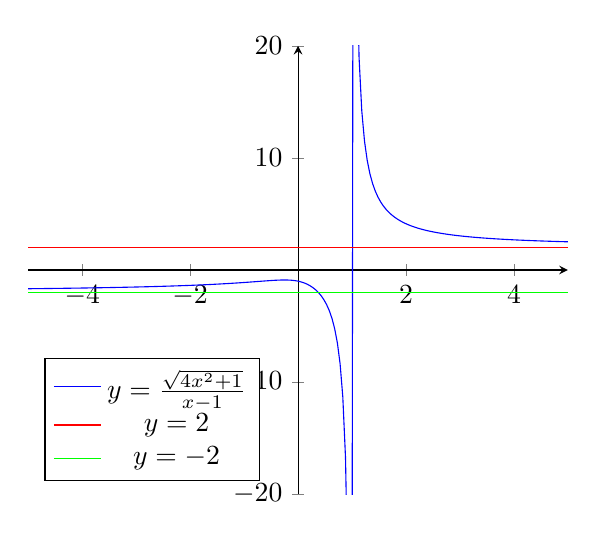
\begin{tikzpicture}
\begin{axis}[axis lines = center, samples = 200, ymin = -20, ymax = 20, legend pos = south west]
\addplot[color = blue]{sqrt(4*x^2 + 1)/(x - 1)};
\addlegendentry{$y = \frac{\sqrt{4x^2 + 1}}{x - 1}$};
\addplot[color = red]{2};
\addlegendentry{$y = 2$};
\addplot[color = green]{-2};
\addlegendentry{$y = -2$};
\end{axis}
\end{tikzpicture}
\end{center}

\newpage

\subsection{Oblique asymptote}
\label{sec:orgcbfb0d6}
The straight line \(y = ax + b, (a \neq 0)\), is an \textbf{oblique asymptote} of the graph of \(y = f(x)\) if:
\[\lim_{x \rightarrow -\infty} (f(x) - (ax + b)) = 0 \quad \text{or} \quad \lim_{x \rightarrow +\infty} (f(x) - (ax + b)) = 0\]

\subsubsection{Example}
\label{sec:org2793db3}
Find the oblique asymptote of:
\[f(x) = \frac{x^3}{x^2 + x + 1}\]

Long divide \(x^3\) by \(x - 1\):
\[f(x) = \frac{x^3}{x^2 + x + 1} = x - 1 + \frac{1}{x^2 + x + 1}\]

So:
\[f(x) - (x - 1) = \frac{1}{x^2 + x + 1} \rightarrow 0 \text{ as } x \rightarrow \pm \infty\]

Hence, \(y = x - 1\) is an oblique asymptote for \(f(x)\).


\section{Relationship between the derivative and monotonicity}
\label{sec:orgf518f5c}
Suppose \(f(x)\) is continuous on \([a, b]\) and differentiable on \((a, b)\). Then:
\begin{itemize}
\item If \(f'(x) > 0\) on \((a, b)\), then \(f\) is strictly increasing on \([a, b]\).
\item If \(f'(x) \ge 0\) on \((a, b)\), then \(f\) is increasing on \([a, b]\).
\item If \(f'(x) < 0\) on \((a, b)\), then \(f\) is strictly decreasing on \([a, b]\).
\item If \(f'(x) \le 0\) on \((a, b)\), then \(f\) is decreasing on \([a, b]\).
\end{itemize}

\newpage

\section{Standard limits}
\label{sec:org790c0d6}
The following equations hold for any numbers \(p > 0\) and \(\varepsilon > 0\):
\[\text{1. } \lim_{x \rightarrow +\infty} \frac{x^p}{e^{\varepsilon x}}\]
\[\text{2. } \lim_{x \rightarrow +\infty} \frac{(\ln x)^p}{x^{\varepsilon}}\]

Rule of thumb:
\begin{itemize}
\item Exponentials beat powers
\item Powers beat logarithms
\end{itemize}


\section{Second derivative and concavity}
\label{sec:org7b6bf2c}
\begin{enumerate}
\item If \(f''(x) > 0\) on an interval \(I\), then \(f\) is \textbf{convex} (or is said to \textbf{concave upward}) on \(I\) (positive means happy face).
\item If \(f''(x) < 0\) on an interval \(I\), then \(f\) is \textbf{concave} (or is said to \textbf{concave downward}) on \(I\) (negative means sad face).
\item If \(a\) is an inflection point for \(f\), then either \(f''(a)\) does not exist, or \(f''(a) = 0\).
\end{enumerate}


\section{Second derivative and extreme points}
\label{sec:org9b25b29}
Suppose \(f \in C^2(I)\), where \(I\) is some open interval containing \(a\), and suppose \(f'(a) = 0\). We have:
\begin{enumerate}
\item If \(f''(a) > 0\), then \(a\) is a point of local minimum.
\item If \(f''(a) < 0\), then \(a\) is a point of local maximum.
\end{enumerate}

Note that if \(f''(a) = 0\), we get no information. \(x = a\) might be a local maximum or minimum or neither.
\end{document}